\newpage
\section{Motivation}
\label {sec:motiv}
%% In this section, we explain the developement process of a highly
%% available application in \tool. We discuss a simple case of anomilies
%% possible under
%% eventual consistency and then explain the difficulties associated 
%% with the ad-hoc anomaly prevention techniques.
%% Lastly we will explain how we generalized and automated such techniques
%% in our tool \tool, and liberated 
%% the developers from all the mentioned problems.
%% Our programming model will be completed in section
%% \ref{sec:ctrt_language}, where we introduce our specification  language,
%% that
%% allows developers fine tune \tool according to \emph{any} 
%% anomaly witnessed in EC stores.
%% %
%% %--- What is the application, what are the requirements 
%
\subsection{Replicated Data Types (RDTs) in Eventually Consistent Stores}
\begin{figure}[t]
        \centering
	\begin{subfigure}[b]{0.489\textwidth}
	\begin{lstlisting}
type Effect = String 
type State =  String 

read :: State -> (String,Maybe Effect)
read s = (s,Nothing)

write :: String -> ((),Maybe Effect)
write comment = ((),comment)

apply :: State -> Effect -> State 
apply s eff = in s ++ " - " ++ comment
	\end{lstlisting}
	\caption{A simple implementation}
	\label{subfig:comment_code}
	\end{subfigure}
	\hfill
	\begin{subfigure}[b]{0.475\textwidth}
	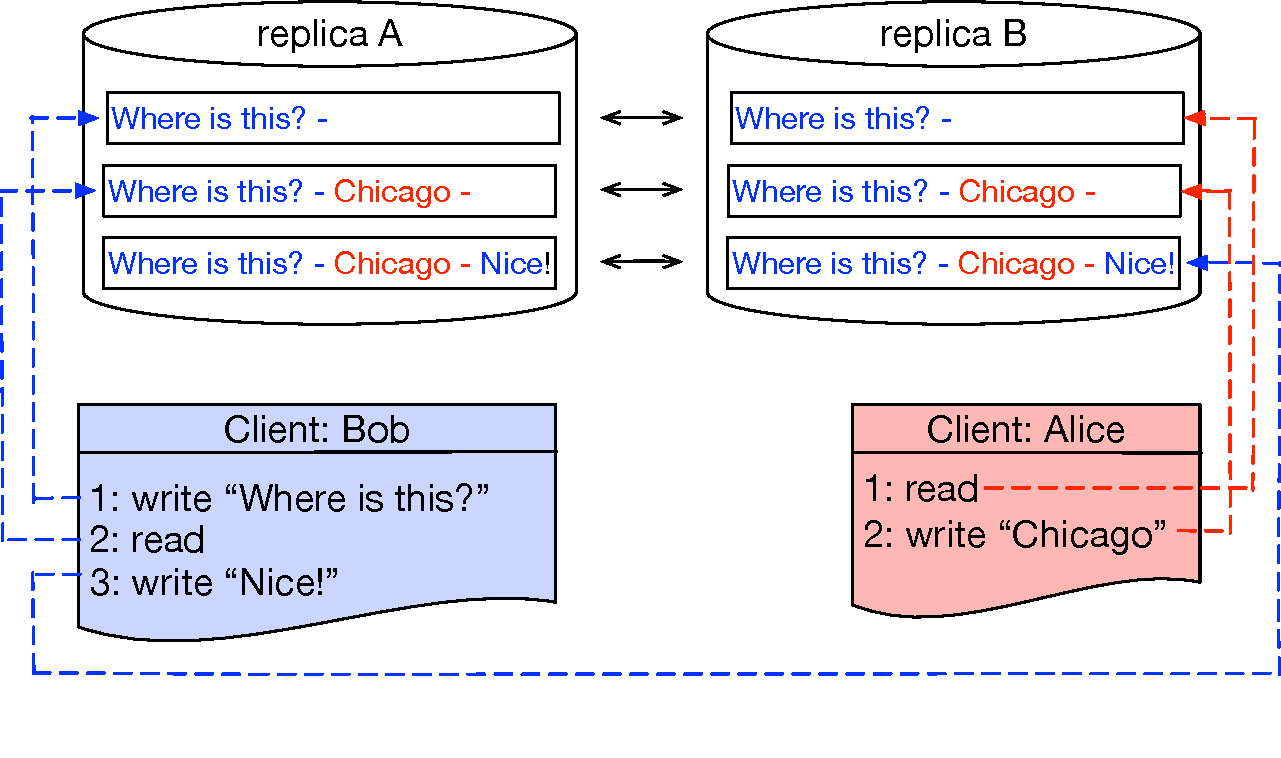
\includegraphics[scale=0.282]{Figures/comment_application.pdf}
	\caption{Example execution}
	\label{subfig:comment_example}
	\end{subfigure} 
\\ \hrulefill
\caption{A distributed application for comment section
management}
\label{fig:comment_app}
\end{figure}




To provide further motivation, consider a highly available (low
latency) application that manages the comment section of posts, as
part of a photo sharing web site.  Fig.~\ref{subfig:comment_code}
presents a simple Haskell implementation of such an application
cognizant of our system model.  The implementation treats
\effectC{} strings as the text of a comment, and 
\stateC{} strings as the concatentation of all visible comments associated
with a post.  A new \effectC{} is generated every time a user wants to
comment on a post by calling the \writeC{} function, and a \readC{}
call simply returns the \stateC{} of the object at the serving
replica.

The \applyC{} function given an effect pastes the included comment to
the end of the current \stateC{}.  For perspicuity, we omit any
conflict resolution strategy in the code; however, developers (using
roll-backs, etc) can design the \applyC{} function to resolve
conflicting concurrent updates as they desire.

Fig. \ref{subfig:comment_example} presents an example of how users
interact with the application. The example shows two clients, Bob and
Alice, that invoke operations on the same object. In the beginning Bob
writes a comment, which is routed to replica A (\ding{182}), whose
effect is then propagated and delivered to replica B (\ding{183});
Alice's first read operation is routed to next (\ding{184}). Alice and
Bob then keep talking through more read and write events while updates
are propagated between replicas, whose order is marked in the figure.

Assume Bob's read operation, instead of being sent to replica A, was
routed to another replica C, where the update from his first operation
was not present. This is known as a \emph{lost-updates} anomaly, a
very well-understood albeit undesirable behavior that is admitted by
eventually consistent stores.  Preventing this sort of anomaly requires
subtle reasoning and may entail sophisticated restructuring of application
logic.

%% Developers are faced with the problem
%% of preventing such an undesired behavior. A task that as we will
%% explain shortly, is difficult, erorneous and heavily tangled with the
%% application logic.
%
%--- What are the challenges implementing those reuquirements manually
%
\subsection{Ad-hoc Anomaly Prevention}
%% In this part, by referring to the modified application  presented in figure
%% \ref{fig:modified_code}, we will
%% explain a well-understood approach toward eliminating the lost-updates anomaly in
%% the  comment manager application dicussed earlier. For simplicity, we
%% assume there are only two clients using the system, Bob and Alice.

%tagging effects
One way to prevent a lost-update anomaly is to \emph{tag} effects and
operations with unique identifiers; such identifiers consist of an
originating session (Alice/Bob), and an integer showing a sequence
number in the session ($line:1,2,3$). This is used by replicas to
record the set of effects they have witnessed.  Tracking dependencies
in this way prevents the anomaly.  Operations that are routed to a
replica that have not witnessed their dependencies are postponed.


%blocking

Another technique called {\bf filtration} is also used to further
realize the above idea, by separating the set of effects that have
arrived to the replica (available effects), and the set of effects
that have arrived and also been applied to the state (filtered
effects).  Replicas can filter the set of available effects before
applying them, so that effects are applied only when all previous
effects, as determined by session order, have been applied.  In order
to maintain the set of all effects applied to the state, replicas
should only record the highest sequence numbers from each session
since it is guaranteed that smaller ones are also already applied
($line:4$).

Fig.~\ref{fig:modified_code} represents the blocking technique in the
modified \readC{} operation, where the result is only returned if the
sequence number of the operation is one larger than the previously
seen sequence number from that session.  ($line:9,11$). Otherwise, the
function is blocked by calling itself recursively ($line:10,12$).
\begin{figure}[t]
	\centering
	\begin{subfigure}[t]{0.5\textwidth}
	\begin{lstlisting}
data Sess = Bob | Alice
type ID = (Sess,Int) 
type Effect= (ID,String)
type State = (String,Int,Int)
	
read :: ID -> State -> String
read (sess,seq) (st,sq1,sq2) = 
	case sess (*@\textcolor{blue}{of}@*) 
		Bob ->   if (seq==sq1+1) (*@\textcolor{blue}{then}@*) st
		         else read (sess,seq)(st,sq1,sq2)
		Alice -> if (seq==sq2+1) (*@\textcolor{blue}{then}@*) st
		         else read (sess,seq)(st,sq1,sq2)
	\end{lstlisting}		  
	\end{subfigure}
	%
	\hfill
        %
	\begin{subfigure}[t]{0.42\textwidth}
	\begin{lstlisting}[firstnumber=13]
	apply :: State -> Effect -> State 
	apply (st,sq1,sq2) ((sess,seq),cm) = 
	  case sess (*@\textcolor{blue}{of}@*) 
	    Bob ->   if (sq1==seq-1)
	             (*@\textcolor{blue}{then}@*) (st++cm,sq1+1,sq2)
	             else (st,sq1,sq2)
	    Alice -> if (sq2==seq-1)
	             (*@\textcolor{blue}{then}@*) (st++cm,sq1,sq2+1)
	             else (st,sq1,sq2)
	\end{lstlisting}		  
        \end{subfigure}

	\hrulefill
	\caption{Guarded Application to Prevent Lost-updates Anomaly
	When Serving Bob and Alice}
	\label{fig:modified_code}
\end{figure}




The above approach obviously requires fundamental and pervasive
changes to the original code.  Additionally, modifications are heavily
tangled with application logic complicating reasoning and hampering
correctness arguments.

Another major drawback of this approach is that it requires constant
alteration to the state of the application when sessions come and go.
Applications are now required to make sure that a new field is created
locally \emph{and} globally when new sessions are connected. This
requires modifying object state in the data store, and making sure
that the global information is updated before allowing local sessions
to start. This requires direct synchronization between replicas,
degrading application performance and availability.

To make the matter worse, new anomalies are constantly found in
systems requiring developers to develop new non-trivial solutions. For
example, in the above application, another type of anomaly can occur
when a third user Chris, uses the application and submits a read,
which is routed to a replica D, that only contains the last write from
Bob. Then Chris sees a window containing "Me too!", which is an
undesirable behavior.  Developers must now either find another ad-hoc
solution, further polluting application logic, or execute the
application using a stronger form of consistency, compromising
performance.

%
%--- What is our alternative approach
%
\subsection{An Alternative}
\begin{wrapfigure}{i}{0.2\textwidth}
\centering
	\vspace{-10mm}
	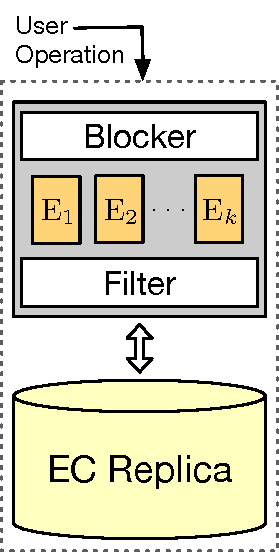
\includegraphics[scale=0.42]{Figures/outline.pdf}
	\label{fig:syncope_outline}
	\caption{\footnotesize \tool}
\label{fig:syncope_outline}
\vspace{-5mm}
\end{wrapfigure}



To overcome these issues, we consider the design of a generic
consistency management tool.  Our goal is to have developers define a
consistency level for each operation \emph{a priori}, ensuring their
satisfiability at runtime. We have realized this idea, following our
observation that preventing anomalies can be expressed in terms of
filtration and blocking.

We therefore propose equipping a distributed data store with a
filtration mechanism that regulates the effects an operation witnesses
(e.g., preventing Chris from seeing Bob's last comment without
including the causal history that preceded it), and a blocking
mechanism that allows operations to execute only when all its
dependent effects have been recorded (e.g., thereby preventing the
lost updates anomaly).  We refer to the view an operation has of a
replica's state as its \emph{environment}.

%% periodically refreshes and allows
%% local effects at the replica to propenter each environment, if their
%% presence would not result in the occurence of the associated
%% anomaly. This way, \tool completely eliminates the possibily of
%% operations \emph{seeing effects that they are not supposed to}, which
%% is one important type of anomalies in distributed systems.  (for
%% example, in the above example Chris was not supposed to see Bob's last
%% comment since some effects were missing from the replica).


%% Similarly, the tool contains a blocker mechanism that makes sure all
%% operations are executed on their associated environment only after the
%% environemnt includes the necessary effects for preventing the associated
%% anomaly. Consequently, the operations will \emph{always see the effects
%% that they are supposed to}. This eliminates another type of anomalies in
%% the distributed systems, that the lost-updates anomaly explained
%% previously, is an
%% example of. 


Our implementation (called \tool) requires developers to specify
constraints on read operations that can be used to synthesize
appropriate filtration and blocking mechanisms.  The specification
language is seeded with $\soZ$ $\visZ$ relations and allows users to
proscribe different anomalous behaviors.  For example, the followings
are the two constraints that prevent the anomalies described above:
the two anomalies mentioned in this section:
\begin{smathpar}
\begin{array}{lllll}

\psi_1: & \forall (\eff,\eff'). & \eff \xrightarrow{\soZ} \eff' & \Rightarrow
& \eff
\xrightarrow {\visZ} \eff'  \\
\psi_2: & \forall(\eff,\eff'). & \eff \xrightarrow{\visZ;\visZ} \eff' &
\Rightarrow & \eff \xrightarrow {\visZ} \eff' 
\end{array}
\end{smathpar}

The specification of the first constraint eliminates the possibility
of lost updates by mandating that any operation \emph{op} with effect
$\eff$ that precedes another \emph{op'} with effect $\eff'$ in session
order must also be visible (i.e., $\eff$ must be witnessed on any
replica that $\emph{op'}$ executes on).  The second specification
prevents causality violations by demanding that if an effect $\eff$ is
visible to another $\eff'$ , then $\eff'$ should also witness any
effects $\eff$ has witnessed.






















